\section{introduzione}
Nell'ambito informatico abbiamo sviluppato un bisogno di organizzare le \emph{informazioni} 
che ci interessano, per poterle semplicemente conservare o \emph{lavorarci}. Il modo 
in cui queste informazioni vengono rappresentate è tramite i \textbf{dati}, quest'ultimi
devono però seguire una certa \textbf{codifica}; vediamo un esempio.

\begin{center}
  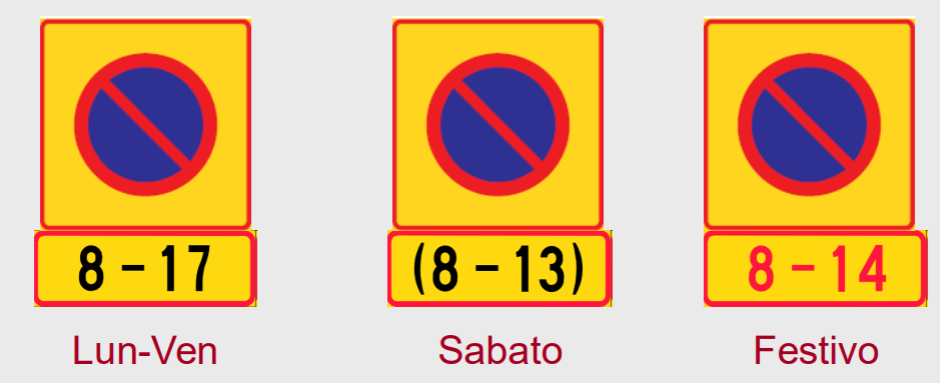
\includegraphics[width=0.5\textwidth]{introduzione/cartelli.png}
\end{center}

I dati che noi estraiamo da questi cartelli (le nostre informazioni) sono gli stessi:
" \emph{divieto dalle 8 alle 17} ". Ma in questo caso la codifica dei dati è molto
importante poichè il modo in cui l'orario viene scritto ci darà \emph{altrettanti} dati. 
Infatti l'orario all'interno delle parentesi indica che riguarda solo il sabato, quello indicato
in rosso è solo nei giorni festivi, senza nessun'altra formattazione invece tutti gli altri giorni.
\\
\\
Per ogni dato dovremmo quindi \emph{specificare} come viene codificato, o semplicemente,
come verrà interpretato, questo può essere un lavoro molto faticoso quando andremo a lavorare
su migliala e milioni di dati. Queste \textbf{basi di dati} verrano allora gestite da un 
\textbf{DBMS}, \textbf{DataBase Management System}. \\
Un \textbf{DBMS} ci permette di gestire con facilità dati di \textbf{grandi} dimensioni (anche
500 Terabyte) e permette di condividere quest'ultimi attraverso più utenti (come tra i vari
settori di una azienda); quest'ultima qualità potrebbe però portare a qualche \textbf{conflitto},
se per esempio dipendente A vuole accedere allo stesso dato su cui sta lavorando dipendente B 
potrebbero formarsi dei dati non accurati. \\
Per questo motivo i \textbf{DBMS} offrono anche meccanismi di autorizzazione, quindi è possibile
definire quale utente è autorizzato a leggere o modificare una certa raccolta di dati.
Un aspetto delicato che deve gestire un \textbf{DBMS} è quindi quello delle \textbf{transizioni},
ovvero tutte quelle operazioni sui dati che devono essere \textbf{atomiche}, ovvero operazioni
non scindibili, devono essere portate a termine per forza di cose, anche nel caso di transizioni
concorrenti (come spiegato prima, quando due utenti operaono sugli stessi dati).